\documentclass[10pt,a4paper,titlepage,croatian]{article}
\usepackage[a4paper]{geometry}
\usepackage{amsmath}
\usepackage{amsfonts}
\usepackage{amssymb}
\usepackage{graphicx} 
\usepackage[utf8x]{inputenc}
\usepackage{listings}
\usepackage[croatian]{babel}
\usepackage{framed}
\usepackage{hyperref}
\usepackage{float}
\usepackage{subfig}
\usepackage{caption}
\usepackage{bookmark}
\usepackage{svg}
%\usepackage{showkeys}
\hypersetup{pdfstartview={XYZ null null 1.00}}
\graphicspath{ {./grafici/} }
\author{Aleksa Marković 2019/0248}
\title{Neuralne mreže - drugi projektni zadatak}
\begin{document}
\lstset{language=Python,breaklines=true} 
\begin{titlepage}
\begin{center}
{\Large Neuralne mreže \par}
\begin{huge}
\sc\textbf{Drugi projektni zadatak}
\par
\end{huge}
\vspace{1cm}
\begin{large}
Aleksa Marković, 2019/0248 \\
Luka Simić, 2019/0368
\\
\vspace{1cm}
Parametri:\\
\vspace{0.5cm}
$V = 5$
\end{large}
\end{center}

\end{titlepage}

\section{Projektovanje}
Opredelili smo se za intuitivni pristup fuzzy upravljanja. Blok dijagram koji smo u projektu napravili može se videti na slici \ref{Simulink}.
% Postupak projektovanja, usvojenu strukturu i konkretno podeˇsavanje parametara

Na početku projektovanja napravili smo blok dijagram koristeći samo step funkciju kao ulazni signal (čije je podešavanje bilo da se promeni sa najmanje reference na najveću), funkciju prenosa zadatu u zadatku, \textit{fuzzy} kontrolerom, povratnom spregom i zakašnjenjem iza funkcije prenosa. Pošto nam je opseg referenci od -2 do 2, to znači da nam je opseg greške od -4 do 4. \textit{Fuzzy} kontroleru bio je zadat \textit{fuzzy inference} sistem sa ulaznom varijablom za grešku (sa 3 funkcije pripadnosti za skupove \texttt{neg}, \texttt{nula} i \texttt{pos}) i izlaznom varijablom za upravljanje (sa 3 funkcije pripadnosti za skupove \texttt{malo}, \texttt{srednje} i \texttt{veliko}).

\begin{figure}[H]
    \centering
    \includesvg[width=\textwidth]{FL_Simulink.svg}
    \caption{\textit{Simulink} blok dijagram korišćen u projektu.}
    \label{Simulink}
\end{figure}

Nakon toga smo u šemu dodali integrator iza \textit{fuzzy} kontrolera, i izmenili izlaz \textit{fuzzy} kontrolera tako da sad vraća brzinu promene upravljanja umesto samog upravljanja (koje je sada na izlazu integratora). Ovde kao vreme koje treba izlaznom signalu da dođe od najmanje do najveće reference uzimamo $\Delta t = 125s$, jer smo poređenjem nekoliko vrednosti (100, 125, 150 i 200 sekundi) ovog vremena na krajnjem stadijumu razvoja FIS zaključili da je za naš problem ova vrednost optimalna. Time dobijamo $\frac{1.2 - (-1.2)}{\Delta t} = 0.0192$, odnosno da je opseg izlaznih vrednosti FIS od -0.0192 do 0.0192 za ovu vrednost $\Delta t$. Ograničenja na izlazu integratora podešena su na ograničenja signala upravljanja, odnosno od -1.2 do 1.2.

Kako bismo rešili problem oscilacija izlaznog signala, dodali smo izvod greške kao ulazni signal u \textit{fuzzy} kontroler (preko saturacije, kako bi osigurala da je greška zaista onakva kakva očekujemo, i multipleksera) i još jednu ulaznu varijablu u FIS za izvod greške sa istim funkcijama pripadnosti kao za grešku i ograničenjem od od -0.1 do 0.1 (dobijeno praćenjem prave vrednosti signala izvoda greške). Tom prilikom u izlaznu varijablu dodajemo još dve funkcije pripadnosti \texttt{srm} i \texttt{srv} koji se koriste u slučaju da je greška 0.

Konačni grafik zavisnosti ulaza od izlaza našeg FIS može se videti na slici \ref{FIS}, dok se parametri funkcija pripadnosti mogu videti u tabelama \ref{in-e}, \ref{in-de} i \ref{out}.

\begin{figure}[H]
    \centering
    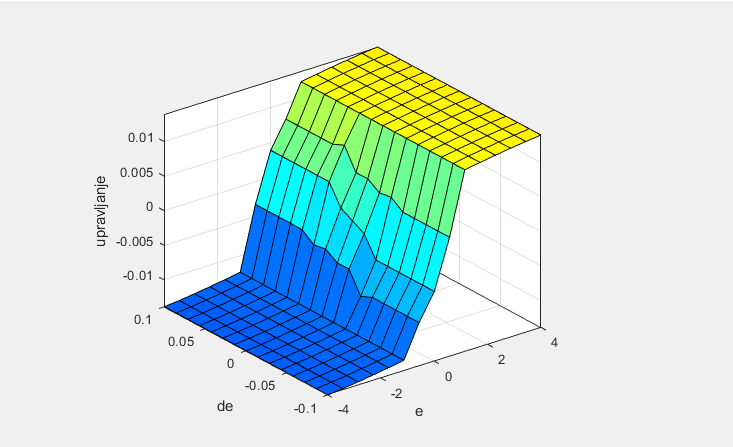
\includegraphics[width=\textwidth]{FL_FIS.png}
    \caption{Grafik zavisnosti ulaza od izlaza \textit{fuzzy inference} sistema.}
    \label{FIS}
\end{figure}

\begin{figure}[H]
    \centering
    \begin{tabular}{|c|c|c|}
        \hline
        Naziv & Tip & Parametri \\
        \hline
        \texttt{neg} & \texttt{trimf} & \texttt{[-5 -4 0]} \\
        \hline
        \texttt{nula} & \texttt{trimf} & \texttt{[-1 0 1]} \\
        \hline
        \texttt{pos} & \texttt{trimf} & \texttt{[0 4 5]} \\
        \hline
    \end{tabular}
    \caption{Postavka parametara ulaza za grešku u FIS.}
    \label{in-e}
\end{figure}

\begin{figure}[H]
    \centering
    \begin{tabular}{|c|c|c|}
        \hline
        Naziv & Tip & Parametri \\
        \hline
        \texttt{neg} & \texttt{trimf} & \texttt{[-0.1834 -0.1 0]} \\
        \hline
        \texttt{nula} & \texttt{trimf} & \texttt{[-0.025 0 0.025]} \\
        \hline
        \texttt{pos} & \texttt{trimf} & \texttt{[0 0.1013 0.25]} \\
        \hline
    \end{tabular}
    \caption{Postavka parametara ulaza za izvod greške u FIS.}
    \label{in-de}
\end{figure}

\begin{figure}[H]
    \centering
    \begin{tabular}{|c|c|c|}
        \hline
        Naziv & Tip & Parametri \\
        \hline
        \texttt{malo} & \texttt{trapmf} & \texttt{[-0.02688 -0.0192 -0.01536 -0.00384]} \\
        \hline
        \texttt{srednje} & \texttt{trimf} & \texttt{[-0.00384 0 0.00384]} \\
        \hline
        \texttt{veliko} & \texttt{trapmf} & \texttt{[0.00376 0.01528 0.01912 0.0384]} \\
        \hline
        \texttt{srm} & \texttt{trimf} & \texttt{[-0.00768 -0.00384 0]} \\
        \hline
        \texttt{srv} & \texttt{trimf} & \texttt{[0 0.00384 0.00768]} \\
        \hline
    \end{tabular}
    \caption{Postavka parametara izlaza FIS.}
    \label{out}
\end{figure}

\section{Rezultati}
Vremenski oblici signala upravljanja, regulisane varijable i signala na neposrednom ulazu mogu se videti na slici \ref{Diagram}.

\begin{figure}[H]
    \centering
    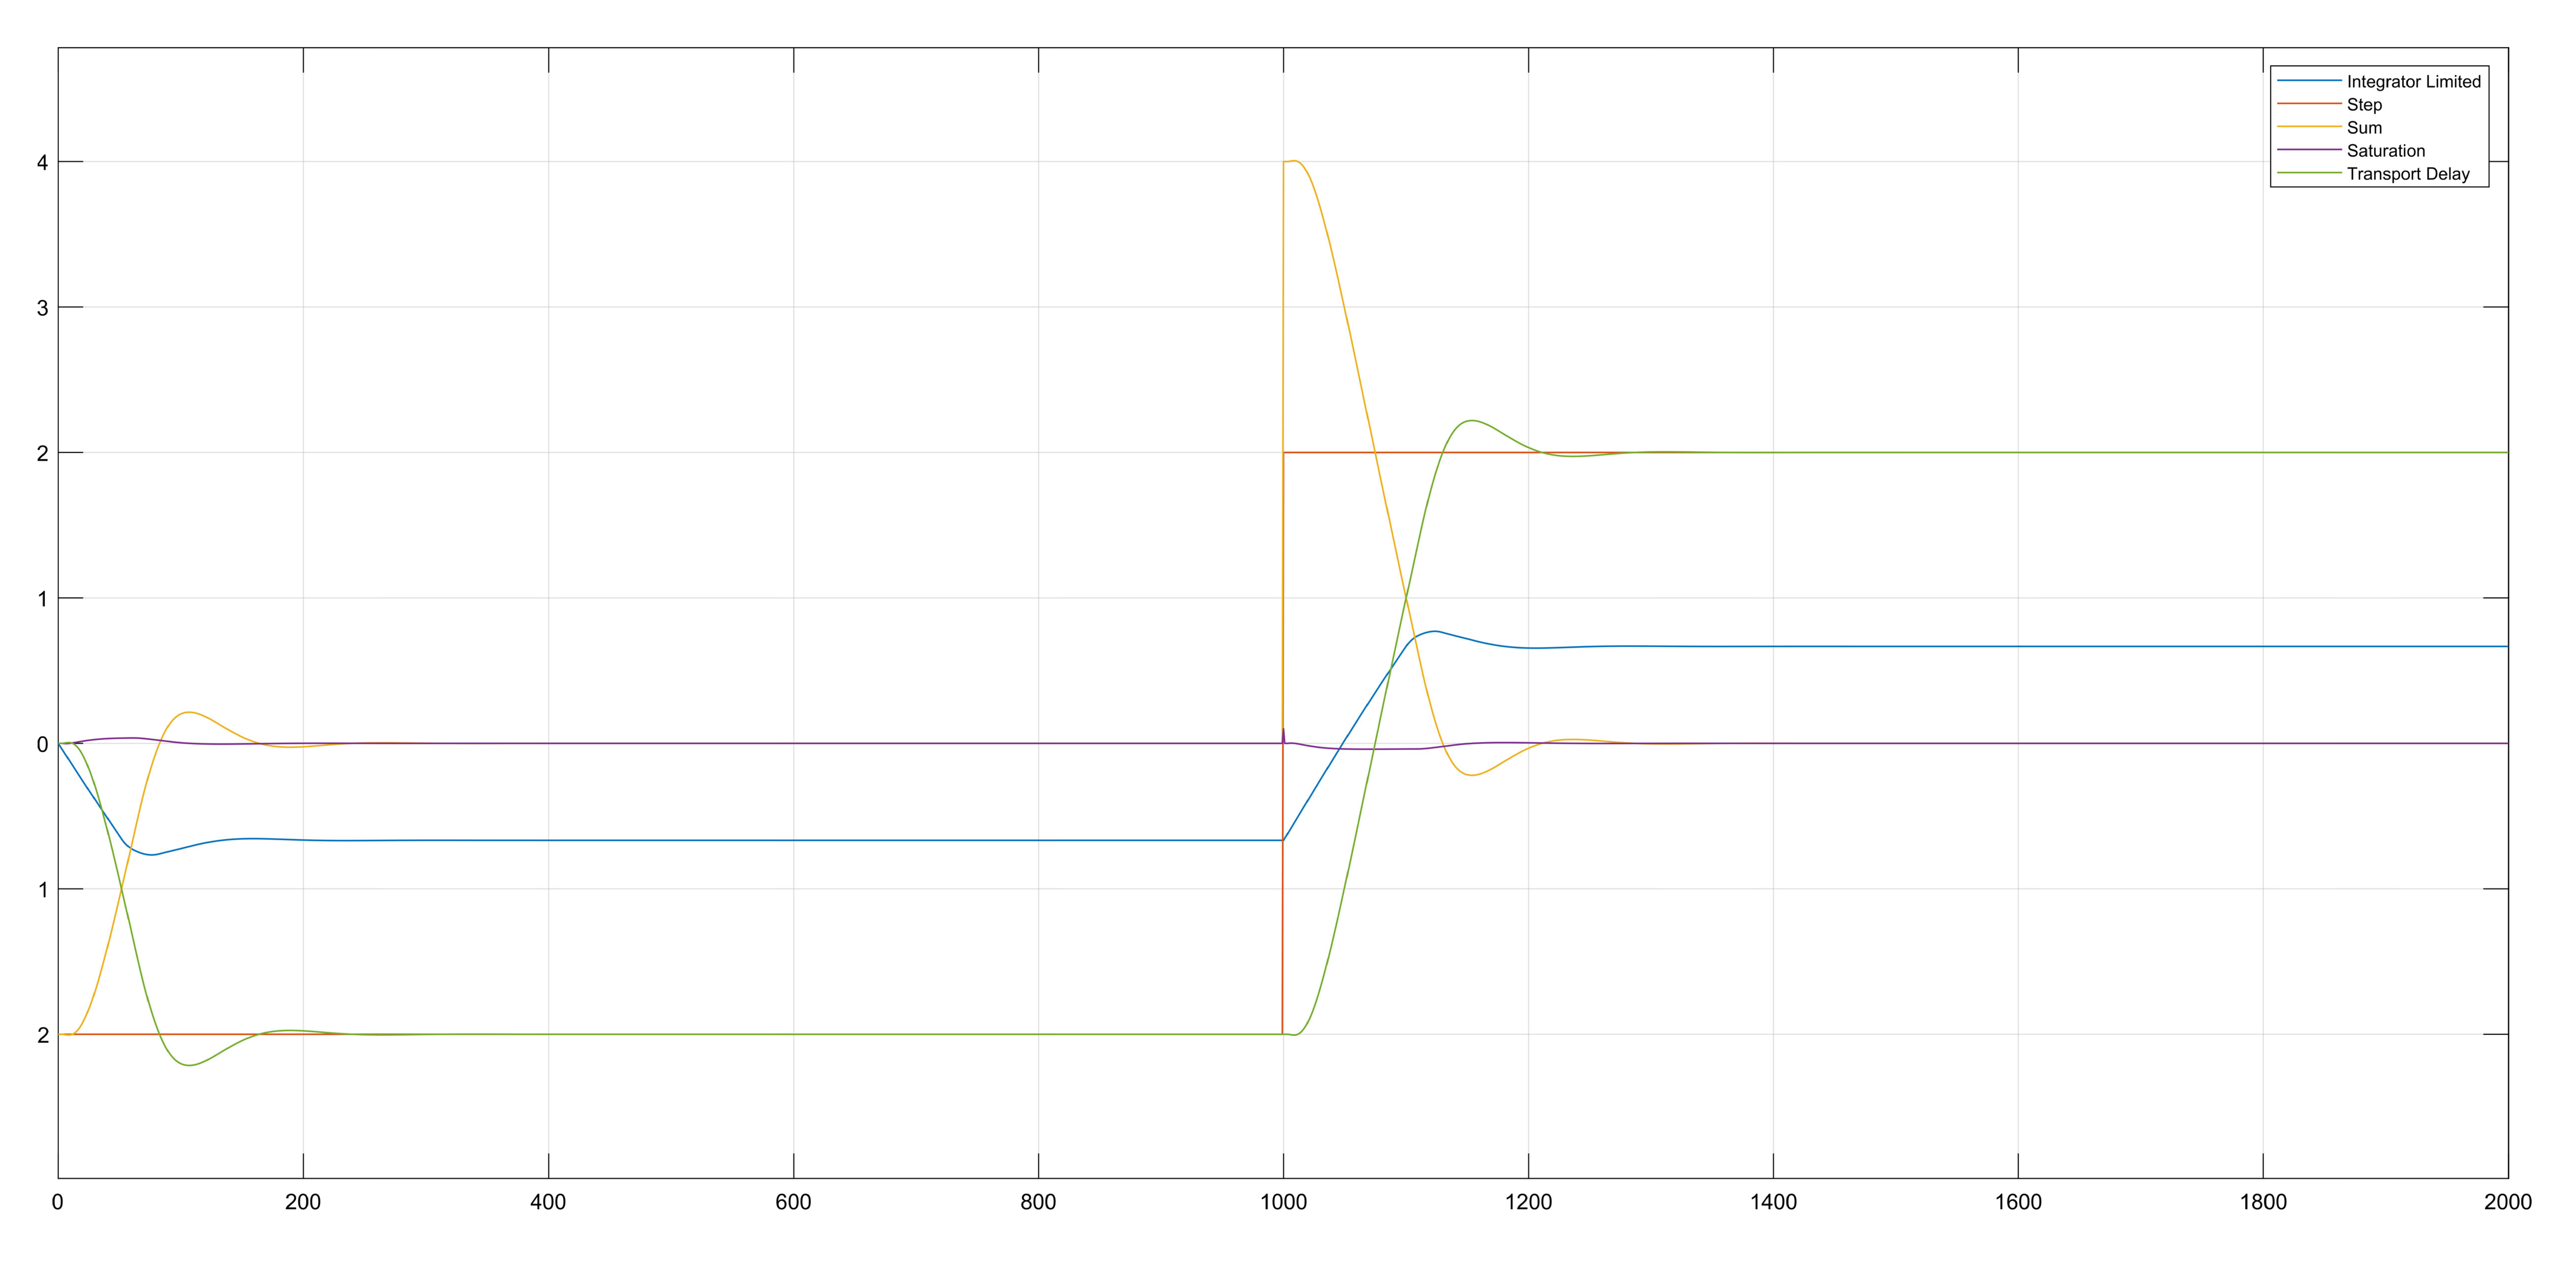
\includegraphics[width=\textwidth]{FL_Diagram.png}
    \caption{Vremenski oblik signala upravljanja, regulisane varijable i signala na neposrednom ulazu.}
    \label{Diagram}
\end{figure}

Izlazna promenljiva se može videti na izlazu Transport Delay. Može se videti jako mali razmak pre nego što izlaz krene da se menja kao rezultat Transport Delay i razmak između podnožja i uspona do reference koji je sličan određenom vremenu $\Delta t$. Može se videti mali preskok kad signal prvi put dostigne referencu nakon skoka sa minimalne na maksimalnu vrednost reference, ali se stabilizacija brže desi zbog diferencijalnog dejstva.

\end{document}
